\section{Experiment Design}\label{sec:experiment}

The most basic meaningful interaction task with a display is to place a cursor
on a target region and ``click'' it to indicate activation intention.  Since
this study was intended to evaluate the efficiency differences in input/output
modalities, we limited it to the most basic ``point and click'' operation
possible: two targets are displayed on the screen at random points along with
a cursor.  The \emph{start} target is initially red and when the user
successfully clicks on it, it turns grey and the \emph{end} target becomes
red.  In the following we refer to each pair of start and end clicks for a
given input/output combination as a \emph{trial}.

Even though real world applications that deal with 3D data often involve dense
scenes with occlusion, it is the authors' anecdotal experience that scenes are
transformed (rotated and translated) by a user prior to interaction in order
to make the desired interaction points congruent with the plane of the screen.
This is equivalent to aligning the axes of the points' principle components
with the screen, which maximizes the accuracy of an input device and the
projected resolution in pixels.  Therefor, we limited the target points to be
randomly generated near the surface of a truncated sphere, such that they were
approximately aligned to the plane of the screen.  This means there is no
occlusion and that the euclidean distance between target points is nearly
constant across all trials.  Randomizing target locations is employed to
prevent motor learning effects as a confound.

We recruited 13 individuals to test on the platform described in the following
section, of which 11 provided suitable data: the first subject revealed flaws
in our test setup, invalidating his results, and another did not complete the
study.  All of the subjects except one are either current students or
professoinals in STEM fields.  Of those whose data was used, the average age
was 26 with 14.6 years of computer use, and 6 were female, 5 male.

Each subject was given a pre-experiment survey (summarized in
\figref{fig:pre_likert}) to ascertain prior familiarity with 3D systems and
interaction, and a post-experiment survey (dicussed further in
below) to provide feedback on the performance and feel of our
test system.  From the pre-survey we see that even though all the subjects are
familiar with computing systems, that their level of experience with 3D
systems and interaction uniformly ranges the gamut from little-to-none
(e.g. has seen the occasional 3D movie or played a video game set in a 3D
world) to highly (e.g. has much experience in 3D design).

\begin{figure}
    \centering
    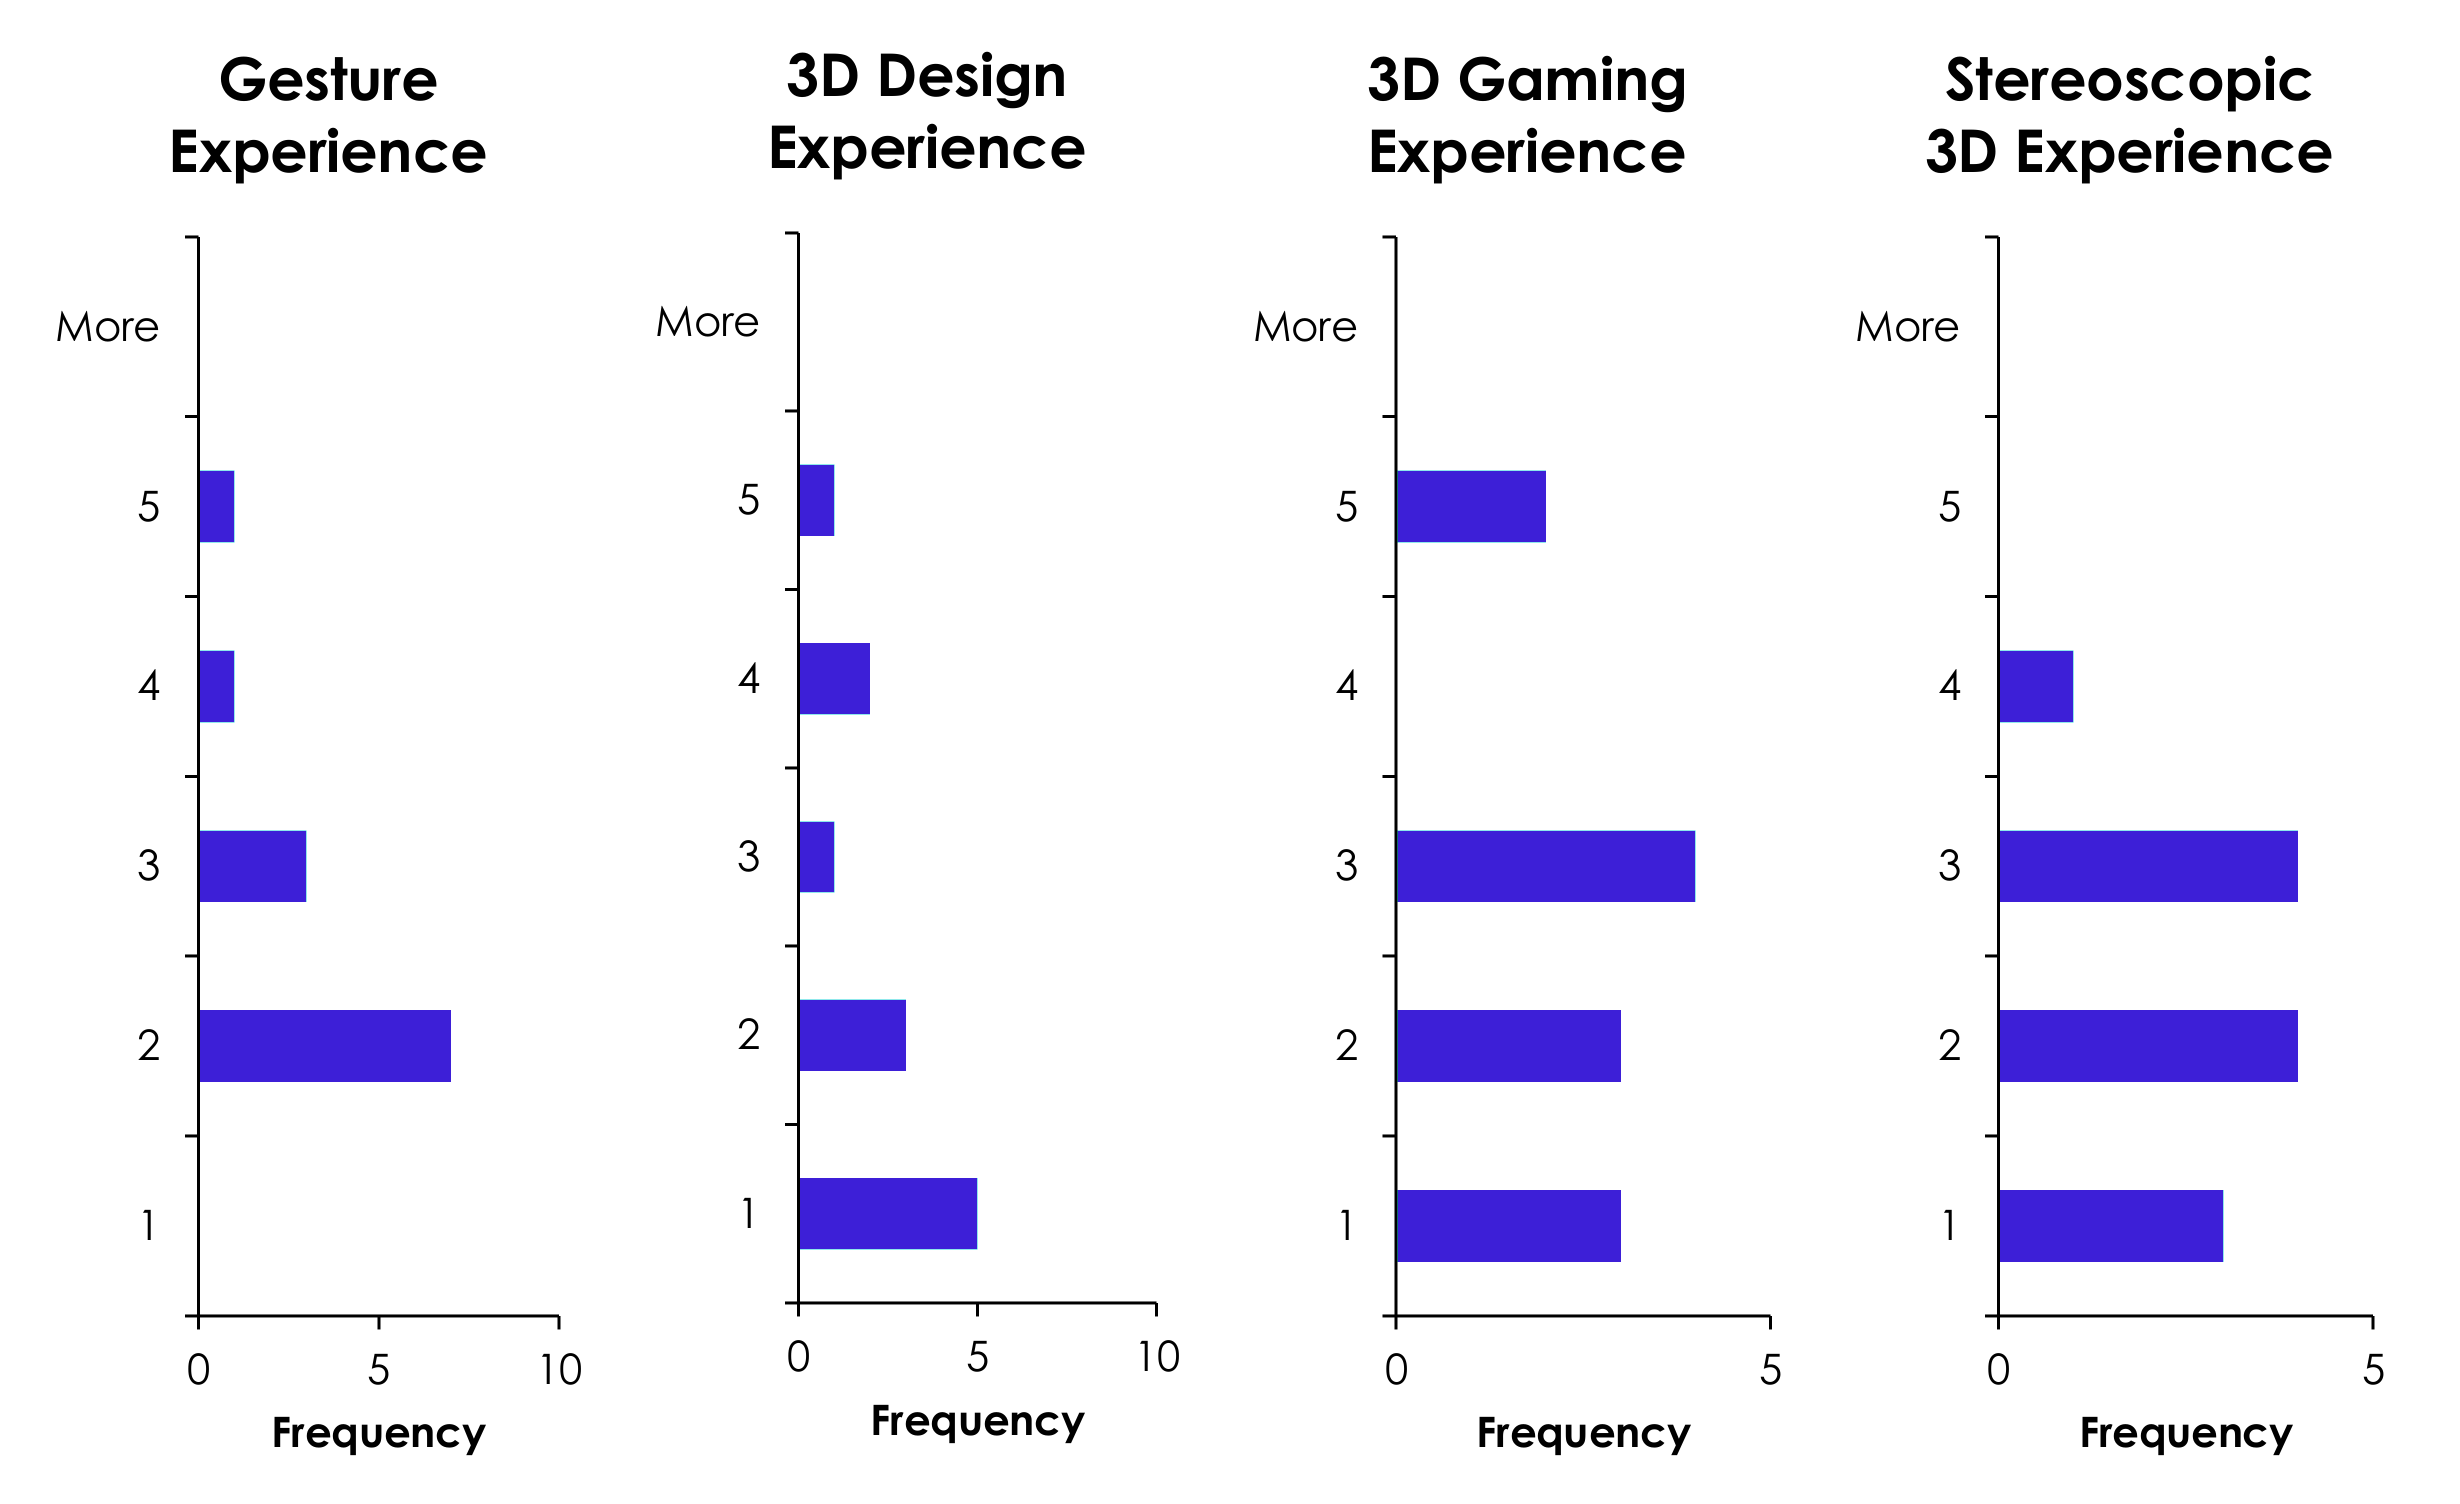
\includegraphics[width=\columnwidth]{pre_likert.png}
    \caption{Pre-experiment responses}
    \label{fig:pre_likert}
\end{figure}

This study was a within-subjects 3x2 design where the input factor has levels
\{Mouse and Keyboard, 3D Mouse, Leap\} and the output factor has levels \{2D
Projections, 3D Headtracked\}.  Each subject was asked to complete 20 trials
for each of the six input/output combination, divided into 12 sessions of 10
trials each.  We used a Latin Square to vary the order of the 12 sessions for
each subject to minimize learning effects from one input/output modality
affecting another.  Prior to starting the 120 trials, each subject was given a
two trial tutorial for each modality.  Subjects were not required to complete
all trials and were informed that they could stop at any time, though only one
chose to stop early (at the halfway point) due to time constraints.  Total
time spent per subject including answering the surveys was around 40 minutes.

We logged cursor pose (3D position and orientation) for each trial at 30Hz for
the duration between clicks on the start and end targets.

